% Convert with command:
% convert -density 300 pic.pdf -quality 90 pic.png
\documentclass[crop,tikz,border=0pt]{standalone}
\usetikzlibrary{arrows.meta}
\usepackage{booktabs}
\begin{document}
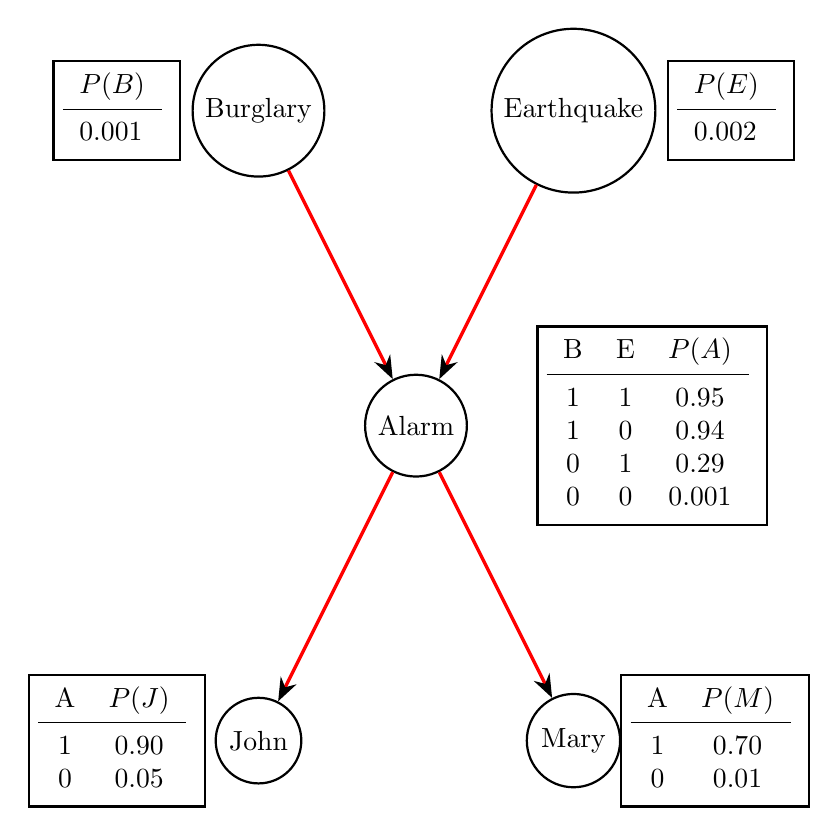
\begin{tikzpicture}

\begin{scope}[every node/.style={circle,thick,draw}]
    \node (A) at (0, 0) [shape=circle, fill=white] {Burglary};
    \node [shape=rectangle,fill=white, align=center](BurglaryTable) at (-1.8, 0) {
            \begin{tabular}{l}
                $P(B)$  \\ \midrule
                0.001
            \end{tabular}
        };
    \node (B) at (4, 0) [shape=circle, fill=white] {Earthquake};
    \node [shape=rectangle,fill=white, align=center](EarthquakeTable) at (6, 0) {
            \begin{tabular}{l}
                $P(E)$  \\ \midrule
                0.002
            \end{tabular}
        };

    \node (C) at (2, -4) [shape=circle, fill=white] {Alarm};
    \node [shape=rectangle,fill=white, align=center](AlarmTable) at (5, -4) {
            \begin{tabular}{ccc} 
                B & E & $P(A)$  \\ \midrule
                1 & 1 & 0.95 \\
                1 & 0 & 0.94 \\
                0 & 1 & 0.29 \\
                0 & 0 & 0.001
            \end{tabular}
        };

    \node (D) at (0, -8) [shape=circle, fill=white] {John};
    \node [shape=rectangle,fill=white, align=center](JohnTable) at (-1.8, -8) {
            \begin{tabular}{cc}
                A & $P(J)$  \\ \midrule
                1 & 0.90 \\
                0 & 0.05
            \end{tabular}
        };
    \node (E) at (4, -8) [shape=circle, fill=white] {Mary};
    \node [shape=rectangle,fill=white, align=center](MaryTable) at (5.8, -8) {
            \begin{tabular}{cc}
                A & $P(M)$  \\ \midrule
                1 & 0.70 \\
                0 & 0.01
            \end{tabular}
        };
\end{scope}


\begin{scope}[>={Stealth[black]},
            %   every node/.style={fill=white,rectangle,above},
              every edge/.style={draw=red,very thick}]
    \path [->] (A) edge node {} (C);
    \path [->] (B) edge node {} (C);
    \path [->] (C) edge node {} (D);
    \path [->] (C) edge node {} (E);
\end{scope}


\end{tikzpicture}
\end{document}
